% Foliensatz: "AFu-Kurs nach DJ4UF" von DK0TU, Amateurfunkgruppe der TU Berlin
% Lizenz: CC BY-NC-SA 3.0 de (http://creativecommons.org/licenses/by-nc-sa/3.0/de/)
% Autoren: Martin Deutschmann

\documentclass[aspectratio=169]{beamer}

\usepackage[ngerman]{babel} % deutsche Worttrennung etc.
\usepackage[utf8]{inputenc} % UTF8 Text

\usepackage[super, comma, numbers, square, sort]{natbib}

\usepackage{hyperref}       % Hyperref Package für bessere Referenzen (todo)
\hypersetup{
	colorlinks=false,       %   false: boxed links; true: colored links
    %linkcolor=white,       %   color of internal links (change box color with linkbordercolor)
    citecolor=red,          %   color of links to bibliography
    filecolor=white,        %   color of file links
    urlcolor=blue           %   color of external links
}

\usepackage{multirow}
\usepackage{wasysym}  % Math Symbols like \permil
%\usepackage{colortbl}
%\usepackage{subscript}
%\usepackage{caption}
%\usepackage{setspace}
%\usepackage{xcolor}        % benutze CodeListe

% Footnote
%\usepackage{hanging}
%
%\setbeamertemplate{footnote}{%
%  \hangpara{2em}{1}%
%  \makebox[2em][l]{\insertfootnotemark}\footnotesize\insertfootnotetext\par%
%}


%\usepackage{pgf}
%\usepackage{tikz}
%\usetikzlibrary{arrows,automata}
%\usetikzlibrary{positioning}
%
%\tikzset{
%    state/.style={
%           rectangle,
%           rounded corners,
%           draw=black, very thick,
%           minimum height=2em,
%           minimum width=2pt,
%           inner sep=2pt,
%           text centered,
%           },
%}

%\usepackage{listings}
%\lstset{basicstyle=\small, numberstyle=\tiny, extendedchars=true, numbers=left, numbersep=5pt}
%\lstset{showtabs=false, showspaces=false, showstringspaces=false}
%%\lstset{backgroundcolor=\color{white!75!lightgray}, , frame=single}
%%\lstset{backgroundcolor=\color{white}}
%%\lstset{backgroundcolor=none}
%\lstset{keywordstyle=\color{blue!50!gray},  identifierstyle=\color{black}}
%\lstset{commentstyle=\color{green!50!gray}, stringstyle=\color{red!50!gray}}
%\lstset{language=C, fontadjust=true, tabsize=2, breaklines=true}
%\lstset{backgroundcolor=\color{white!75!lightgray}, caption=\lstname, frame=single}
%\lstset{emphstyle=\color{black}\fbox}
%
%% Keine "Listing:"-Caption
%\captionsetup{labelformat=empty,labelsep=none}
%
%% für mathematische Umgebungen
%\usepackage{amsmath,amsfonts,amssymb}
%
%\lstdefinestyle{Bash}{
%language=Bash,
%frame=single,
%rulecolor=\color{black},
%backgroundcolor=\color{gray!50},
%keywordstyle=\color{black},
%identifierstyle=,
%commentstyle=\color{black},
%stringstyle=\color{magenta!65!white},
%showstringspaces=false,
%basicstyle=\footnotesize\ttfamily\color{black},
%numbers=none,
%breaklines=true,
%captionpos=b
%}

%\usepackage{listings}
%
%\lstdefinestyle{basic}{
%    captionpos=t,%
%    basicstyle=\footnotesize\ttfamily,%
%    numberstyle=\tiny,%
%    numbers=left,%
%    stepnumber=1,%
%    frame=single,%
%    showspaces=false,%
%    showstringspaces=false,%
%    showtabs=false,%
%    %
%    keywordstyle=\color{blue},%
%    identifierstyle=,%
%    commentstyle=\color{gray},%
%    stringstyle=\color{magenta}%
%}



% fließende Boxen haben keinen Abstand
%\fboxsep0mm

% inkludiere Creative Commons Helper
%%%%%%%%%%%%%%%%%%%%%%%%%%%%%%%%%%%%%%%%%%%%%%%%%%%%%%%%%%%%%%%%
%% ccBeamer 0.1, 2007-07-02                                   %%
%% Written by Sebastian Pipping <webmaster@hartwork.org>      %%
%% ---------------------------------------------------------- %%
%% Licensed under Creative Commons Attribution-ShareAlike 3.0 %%
%% http://creativecommons.org/licenses/by-sa/3.0/             %%
%%%%%%%%%%%%%%%%%%%%%%%%%%%%%%%%%%%%%%%%%%%%%%%%%%%%%%%%%%%%%%%%


%% Images
\newcommand{\CcImageBy}[1]{%
	
\includegraphics[scale=#1]{texdata/creative_commons/cc_by_30.pdf}%
}
\newcommand{\CcImageCc}[1]{%
	
\includegraphics[scale=#1]{texdata/creative_commons/cc_cc_30.pdf}%
}
\newcommand{\CcImageDevNations}[1]{%
	
\includegraphics[scale=#1]{texdata/creative_commons/cc_dev_nations_30.pdf}%
}
\newcommand{\CcImageNc}[1]{%
	
\includegraphics[scale=#1]{texdata/creative_commons/cc_nc_30.pdf}%
}
\newcommand{\CcImageNd}[1]{%
	
\includegraphics[scale=#1]{texdata/creative_commons/cc_nd_30.pdf}%
}
\newcommand{\CcImagePd}[1]{%
	
\includegraphics[scale=#1]{texdata/creative_commons/cc_pd_30.pdf}%
}
\newcommand{\CcImageSa}[1]{%
	
\includegraphics[scale=#1]{texdata/creative_commons/cc_sa_30.pdf}%
}
\newcommand{\CcImageSampling}[1]{%
	
\includegraphics[scale=#1]{texdata/creative_commons/cc_sampling_30.pdf}%
}
\newcommand{\CcImageSamplingPlus}[1]{%
	
\includegraphics[scale=#1]{texdata/creative_commons/cc_sampling_plus_30.pdf}%
}


%% Groups
\newcommand{\CcGroupBy}[2]{% zoom, gap
	\CcImageCc{#1}\hspace*{#2}\CcImageBy{#1}%
}
\newcommand{\CcGroupByNc}[2]{% zoom, gap
	\CcImageCc{#1}\hspace*{#2}\CcImageBy{#1}\hspace*{#2}\CcImageNc{#1}%
}
\newcommand{\CcGroupByNcNd}[2]{% zoom, gap
	\CcImageCc{#1}\hspace*{#2}\CcImageBy{#1}\hspace*{#2}\CcImageNc{#1}\hspace*{#2}\CcImageNd{#1}%
}
\newcommand{\CcGroupByNcSa}[2]{% zoom, gap
	\CcImageCc{#1}\hspace*{#2}\CcImageBy{#1}\hspace*{#2}\CcImageNc{#1}\hspace*{#2}\CcImageSa{#1}%
}
\newcommand{\CcGroupByNd}[2]{% zoom, gap
	\CcImageCc{#1}\hspace*{#2}\CcImageBy{#1}\hspace*{#2}\CcImageNd{#1}%
}
\newcommand{\CcGroupBySa}[2]{% zoom, gap
	\CcImageCc{#1}\hspace*{#2}\CcImageBy{#1}\hspace*{#2}\CcImageSa{#1}%
}
\newcommand{\CcGroupDevNations}[2]{% zoom, gap
	\CcImageCc{#1}\hspace*{#2}\CcImageDevNations{#1}%
}
\newcommand{\CcGroupNcSampling}[2]{% zoom, gap
	\CcImageCc{#1}\hspace*{#2}\CcImageNc{#1}\hspace*{#2}\CcImageSampling{#1}%
}
\newcommand{\CcGroupPd}[1]{% zoom
	\CcImagePd{#1}%
}
\newcommand{\CcGroupSampling}[1]{% zoom
	\CcImageSampling{#1}%
}
\newcommand{\CcGroupSamplingPlus}[1]{% zoom
	\CcImageSamplingPlus{#1}%
}


%% Text
\newcommand{\CcLongnameBy}{Attribution}
\newcommand{\CcLongnameByNc}{Attribution-NonCommercial}
\newcommand{\CcLongnameByNcNd}{Attribution-NoDerivs}
\newcommand{\CcLongnameByNcSa}{Attribution-NonCommercial-ShareAlike}
\newcommand{\CcLongnameByNd}{Attribution-NoDerivs}
\newcommand{\CcLongnameBySa}{Attribution-ShareAlike}

\newcommand{\CcNote}[1]{% longname
	This work is licensed under the \textit{Creative Commons #1 3.0 License}.%
}


% generelles Thema auswählen
\usetheme{Goettingen} %Berlin spart ohne Sidebar allerdings angenehm Platz
% AnnArbor | Antibes | Bergen | Berkeley | Berlin | Boadilla | boxes | CambridgeUS | Copenhagen | Darmstadt | default | Dresden | Frankfurt | Goettingen | Hannover | Ilmenau | JuanLesPins | Luebeck | Madrid | Malmoe | Marburg | Montpellier | PaloAlto | Pittsburgh | Rochester | Singapore | Szeged | Warsaw

% Farben wählen
\usecolortheme{beetle}
% beaver | beetle | crane | default | dolphin | dove | fly | lily | orchid | rose | seagull | seahorse | sidebartab | structure | whale | wolverine

% Setze alle Farben auf Grau und Weiß
%\definecolor{craneorange}{RGB}{64,64,64}
%\definecolor{craneblue}{RGB}{255,255,255}

% Schriftart wählen
\usefonttheme{default}
% default | professionalfonts | serif | structurebold | structureitalicserif | structuresmallcapsserif

% Innere Themen(Kopf-, Fuß-, Sidebar usw)
%\useinnertheme{default}
\useinnertheme{circles}
% default | inmargin | rectangles | rounded | circles

% Äußere Themen (Anordnung der inneren, grenzen der Folien etc.)
\useoutertheme{infolines}
% default | infolines | miniframes | shadow | sidebar | smoothbars | smoothtree | split | tree

% Deaktiviere Navigations-Symbole ({} -> leer)
\setbeamertemplate{navigation symbols}{}
%\setbeamertemplate{navigation symbols}{\large \ifnum \insertframenumber <10 0\fi\insertframenumber/\inserttotalframenumber\vspace*{0.2ex}}

% Zeige ein Hintergrundbild
\setbeamertemplate{background canvas}{
        \hspace*{-2.0cm}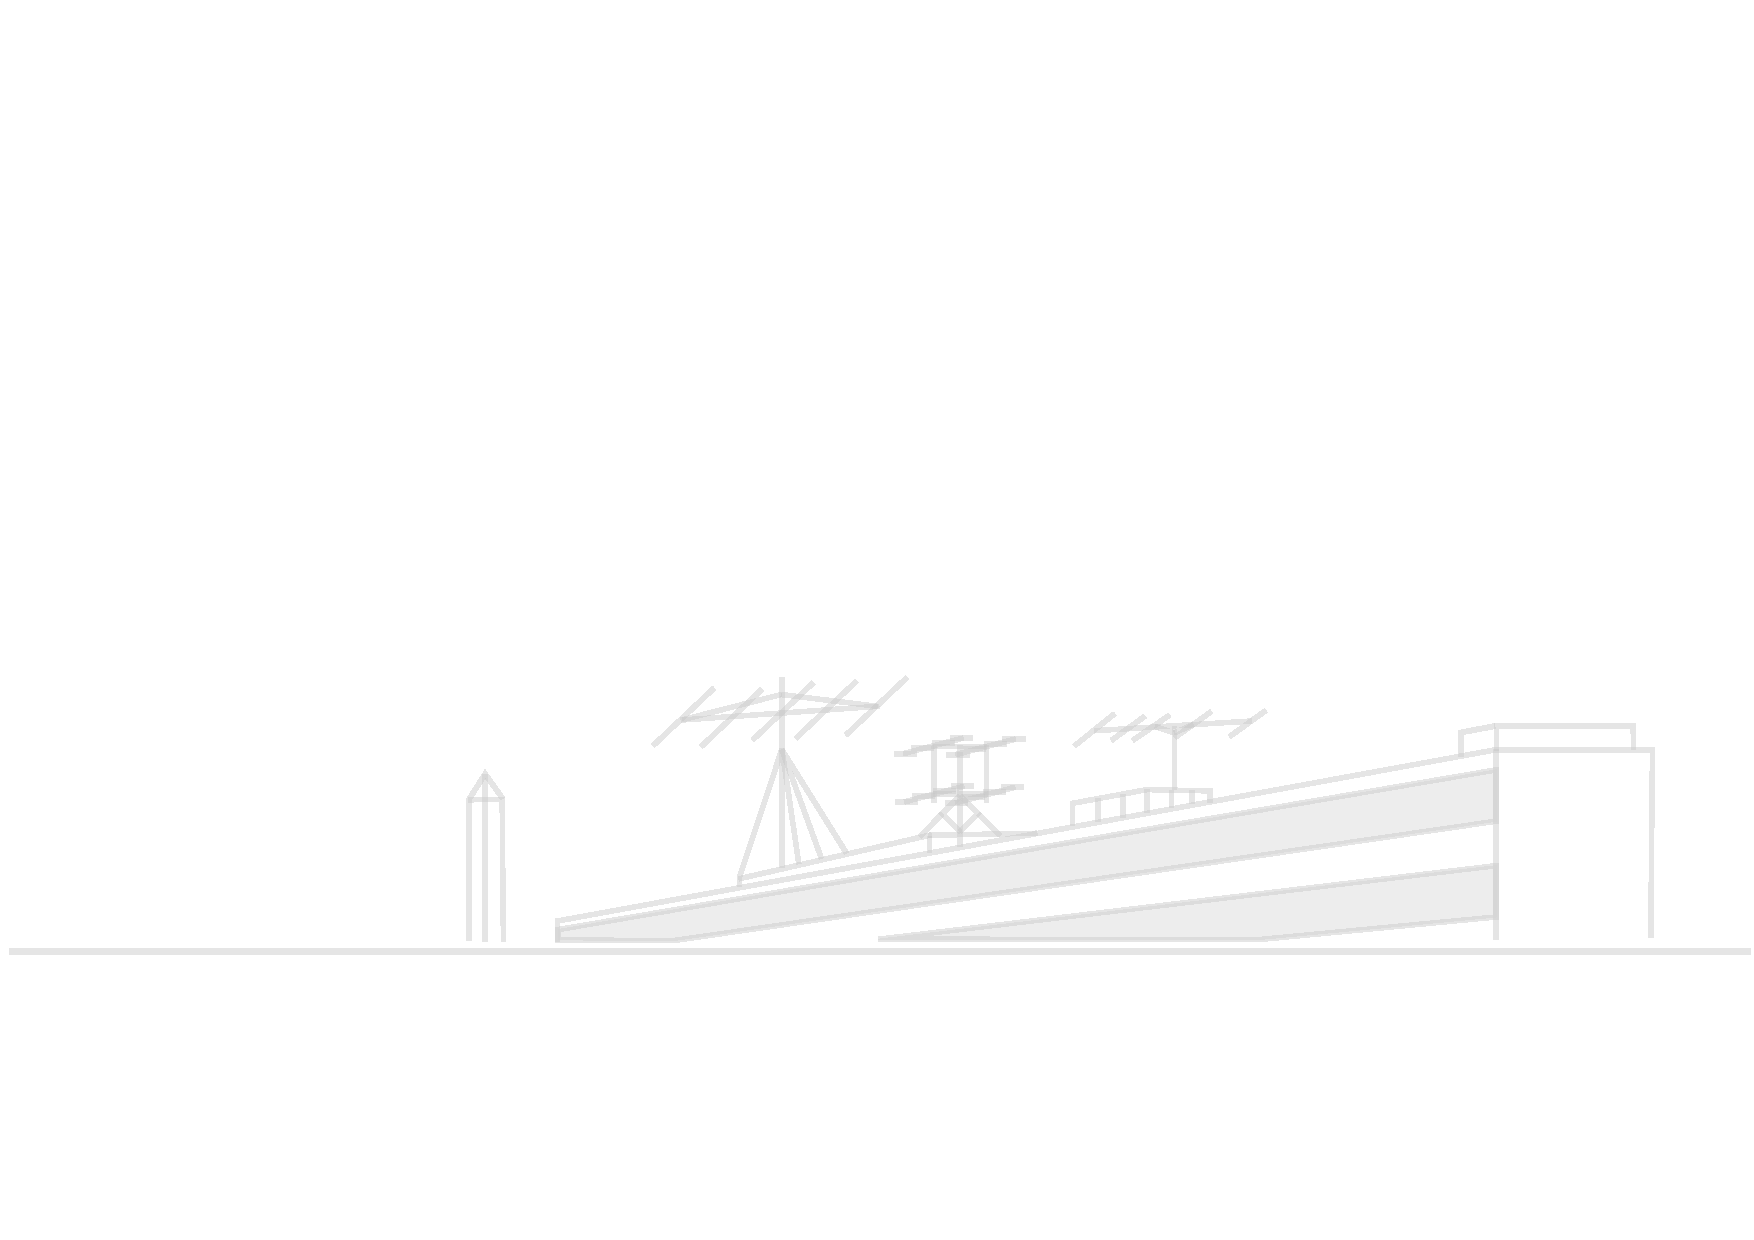
\includegraphics[width=17.8cm]{texdata/dk0tu_rooftop_background.pdf}
}

% Foliennummer einfügen
\setbeamertemplate{footline}[frame number]
%\setbeamertemplate{footline}{}

% Ändere das Zeichen vor jedem item
%\setbeamertemplate{itemize item}{\color{craneorange}$\blacktriangleright$}
%\setbeamertemplate{itemize subitem}{\color{craneorange}$\triangleright$}
%\setbeamertemplate{itemize subsubitem}{\color{craneorange}$\blacktriangleright$}

% Ändert die Blöcke 
\setbeamertemplate{blocks}[rounded][shadow=true]
% default | rounded [shadow=true|false]

%
% Eigene Kommandos
%

% Hack to get natbib and beamer working together. "The beamer user guide suggests
% that only the manual bibliography entry approach is supported"
% on some system it works out of the box, sometimes you need the hack :-(
% so check it --dl7bst
\ifdefined\newblock
    \relax
\else
    \newcommand{\newblock}{}
\fi

% \includedia command to generate png out of a dia file
% NEEDS installed dia and pdflatex option --shell-escape
\newcommand{\includedia}[1]{
    \immediate\write18{/usr/bin/dia #1.dia -e #1_diatmp.png -t png}
}

% RICHIG GROSSER FONT!
\newfont{\bigfont}{cmr10 at 144pt}
\newfont{\smallfont}{cmr10 at 8pt}

% Römische Ziffern
\makeatletter
\newcommand{\rmnum}[1]{\romannumeral #1}
\newcommand{\Rmnum}[1]{\expandafter\@slowromancap\romannumeral #1@}
\makeatother

% Schwarze Überschrift
%\setbeamercolor{frametitle}{fg=black}
%\setbeamercolor{title}{fg=black}

% Item- und Box-Farben
\definecolor{deepBlue}{HTML}{000066}
\setbeamercolor{itemize item}{fg=deepBlue}
\setbeamercolor{itemize subitem}{fg=deepBlue}
\setbeamercolor{description item}{fg=deepBlue}
\setbeamercolor{block title}{fg=deepBlue!100, bg=blue!15}
\setbeamercolor{block body}{fg=black, bg=blue!5}
\setbeamercolor{block title alerted}{fg=deepBlue, bg=red!75}
\setbeamercolor{block body alerted}{fg=black, bg=red!15}
\setbeamercolor*{block title example}{fg=blue!50, bg=blue!10}
\setbeamercolor*{block body example}{fg= blue, bg=blue!5}

%\setbeamercolor{section in head/foot}{parent=palette primary}
%\setbeamercolor{subsection in head/foot}{parent=palette secondary}
%\setbeamercolor{sidebar}{fg=darkblue,bg=yellow!90!orange}
%\setbeamercolor{title in sidebar}{fg=darkblue}
%\setbeamercolor{author in sidebar}{fg=darkblue}
%\setbeamercolor{section in sidebar}{fg=darkblue!10!black}
%\setbeamercolor{subsection in sidebar}{fg=darkblue!50!black}

% Titlepage Infos
\title{AFu-Kurs nach DJ4UF}
\author[DKØTU]{DKØTU\\ \footnotesize{Amateurfunkgruppe der TU Berlin}}
\institute[DKØTU]{\url{http://www.dk0tu.de} }

% PDF-Eigenschaften
\subject{DK0TU-Amateurfunkkurs nach DJ4UF}
\keywords{Amateurfunk Kurs HAM Radio Course CC-BY-NC-SA OpenSource TU Berlin DK0TU}

\subtitle{Technik Klasse E 10: \\
          Dezibel, D\"ampfung \& Kabel \\[2em]}
\date{Stand 01.12.2014}
 \begin{document}

\begin{frame}
    \titlepage
    \vfill
    \begin{center}
        \ccbyncsaeu\\
        {\tiny This work is licensed under the \em{Creative Commons Attribution-NonCommercial-ShareAlike 3.0 License}.}\\[0.5ex]
         \tiny Amateurfunkgruppe der Technische Universität Berlin (AfuTUB), DKØTU
         %\includegraphics[scale=0.5]{img/DK0TU_Logo.pdf}
    \end{center}
\end{frame}


%fixme Referenzen/Fußnoten-Systematik vereinheitlichen

\section*{D\"ampfungsfaktor}
\begin{frame}
\frametitle{D\"ampfungsfaktor}
\begin{center}
\begin{minipage}{0.3\textwidth}
	\huge{$ D = \frac{P_{1}}{P_{2}}$}
\end{minipage}
\begin{minipage}{0.6\textwidth}
\begin{itemize}
	\item  D\"ampfungsfaktor D gibt Verh\"altnis zwischen Eingangsleistung $P_{1}$ und der Ausgangsleistung $P_{2}$.
\end{itemize}	
\end{minipage}
\vspace{1cm}	
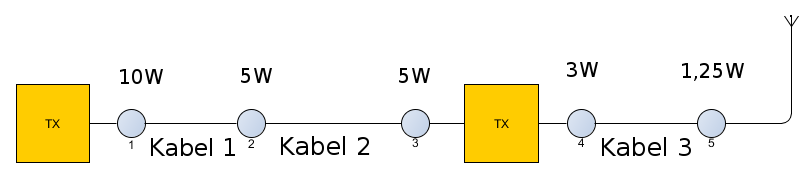
\includegraphics[scale=0.35]{e10/ubertragung.png}\\
Abb. 1: Übertragungswege einer Funkstation
\end{center}
\end{frame}



\section*{D\"ampfungsma{\ss} dB}
\begin{frame}
\frametitle{D\"ampfungsma{\ss} dB}
\begin{center}
	\begin{itemize}
		\item D\"ampfungsma{\ss} ist die logarithmierung des D\"ampfungsfaktor
		\item logarithmische Werte kann man addieren
	\end{itemize}
	\vspace{0.5cm}
	\fbox{
		\Huge{$a_{P} = 10 \cdot log(\frac{P_{1}}{P_{2}})$ dB}
	}
\end{center}
\end{frame}

\section{Verst\"arkung in dB}
\begin{frame}
\frametitle{Verst\"arkung in dB}
\begin{itemize}
	\item im Amateurfunk wird mit Verstärkung und nicht mit D\"ampfung gerechnet
	\item D\"ampfung ist eine negative Verst\"arkung
\end{itemize}
\vspace{1cm}
	\fbox{
		\Huge{$g = 10 \cdot log(\frac{P_{2}}{P_{1}})$ dB}
	}
\end{frame}

\begin{frame}
\frametitle{Verst\"arkung in dB}
\begin{center}
	\begin{Large}
	\begin{tabular}{|c|c|}
		\hline
		dB & Leistungsfaktor \\
		\hline \hline
		0    & 1                 \\ \hline
		1,5  & $\sqrt{2}$ = 1,41 \\ \hline
		2,15 & 1,64              \\ \hline
		3    & 2                 \\ \hline
		6    & 4                 \\ \hline
		10   & 10                \\ \hline
		20   & 100               \\ \hline
	\end{tabular}
	\end{Large}		
	\end{center}
\end{frame}

\section*{Spannungsd\"ampfungsma{\ss}}
\begin{frame}
\frametitle{Spannungsd\"ampunfgsma{\ss}}
\fbox{
		\Huge{$a_{U} = 20 \cdot log(\frac{U_{1}}{U_{2}})$ dB}
	}
\vspace{2cm}
\begin{itemize}
	\item Wird in der A-Technik n\"aher erl\"autert.
\end{itemize}
\end{frame}

\begin{frame}
\frametitle{Spannungsfaktor \& Leistungsfaktor}
\begin{center}
\begin{Huge}
\begin{minipage}{0.3\textwidth}
	\begin{tabular}{|c|c|}
		\hline
		dB & $a_{U}$ \\
		\hline \hline
		6dB  & 2  \\ \hline
		12dB & 4  \\ \hline
		20dB & 10 \\ \hline
	\end{tabular}
\end{minipage}
\hspace{2cm}
\begin{minipage}{0.3\textwidth}
	\begin{tabular}{|c|c|}
		\hline
		dB & $a_{P}$ \\
		\hline \hline
		3dB  & 2  \\ \hline
		6dB  & 4  \\ \hline
		10dB & 10 \\ \hline
	\end{tabular}
\end{minipage}
\end{Huge}
\end{center}
\end{frame}

\section*{S-Stufen}
\begin{frame}
\frametitle{S-Stufen}
\begin{center}
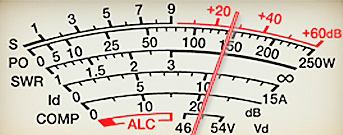
\includegraphics[scale=1.2]{e10/S-Meter.jpg}\\
Abb. 2: S-Meter
\footnote{\url{http://commons.wikimedia.org/wiki/File:S-Meter.jpg}}
\begin{itemize}
	\item eine S-Stufe entspricht 6 dB
	\item Wird beim RST-System verwendet
	\item gibt einen bestimmten Spannungswert an einem 50$\Omega$ Widerstand an
	\item Kurzwelle: S9 = 50$\mu$V bei 50$\Omega$
	\item UKW: S9 = 5$\mu$V bei 50$\Omega$
\end{itemize}
\end{center}
\end{frame}

\section*{Pegel}
\begin{frame}
\frametitle{Pegel}
\begin{center}
\begin{large}
\begin{minipage}{0.3\textwidth}
	\begin{tabular}{|c|c|}
		\hline
		dBm & mW \\
		\hline \hline
		20dBm  & 100mW  \\ \hline
		10dBm  & 10mW   \\ \hline
		0dBm   & 1mW    \\ \hline
		-10dBm & 0,1mW  \\ \hline
	\end{tabular}
\end{minipage}
\hspace{2cm}
\begin{minipage}{0.3\textwidth}
	\begin{tabular}{|c|c|}
		\hline
		dBpW & mW \\
		\hline \hline
		20dBpW  & 100pW  \\ \hline
		10dBpW  & 10pW   \\ \hline
		0dBpW   & 1pW    \\ \hline
		-10dBpW & 0,1pW  \\ \hline
	\end{tabular}
\end{minipage}
\vspace{0.5cm}
\end{large}
\begin{itemize}
	\item Pegel ist auf einen bestimmten Grundwert bezogen
	\item Grundwert wird auch Normal oder Nullwert genannt
\end{itemize}
\end{center}
\end{frame}


\section*{Hochfrequenzleitung}
\begin{frame}
\frametitle{Hochfrequenzleitungen}
\begin{center}
%\begin{minipage}{0.4\textwidth}
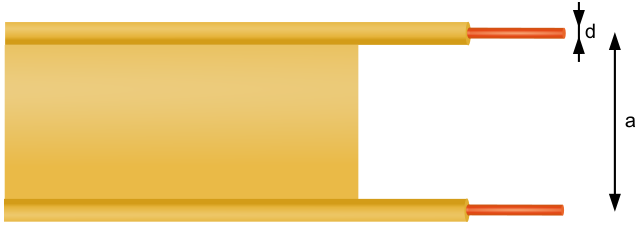
\includegraphics[scale=0.25]{e10/parallel.png}\\
\footnote{\url{http://de.wikipedia.org/wiki/Datei:Twin-lead_cable_dimension.svg}}
Abb. 3: Paralleldrahtleitung
%\end{minipage}\\
\\
%\begin{minipage}{0.4\textwidth}
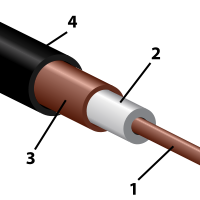
\includegraphics[scale=0.4]{e10/coax.png}\\
\footnote{\url{http://commons.wikimedia.org/wiki/File:Coaxial_cable_cutaway_new.svg}}
Abb. 4: Koaxialkabel
%\end{minipage}
\end{center}
\end{frame}

\section*{Hochfrequenzleitung}
\begin{frame}
\frametitle{Hochfrequenzleitungen}
\begin{center}
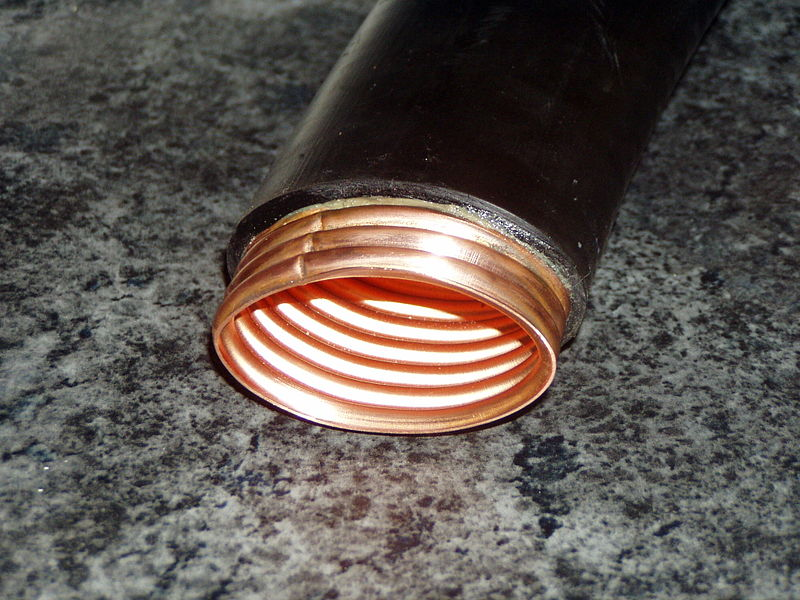
\includegraphics[scale=0.4]{e10/hohl.jpg}\\
\footnote{\url{http://de.wikipedia.org/wiki/Datei:Elli_holl.jpg}}
Abb. 5: Hohlleiter
%\end{minipage}
\end{center}
\end{frame}

\section*{Wellenwiderstand}
\begin{frame}
\frametitle{Wellenwiderstand}
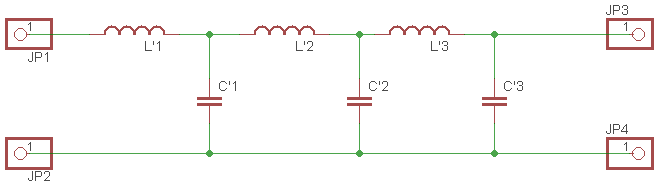
\includegraphics[scale=0.8]{e10/wellenesb.png}\\
Abb. 6: ESB 
\vspace{1cm}\\
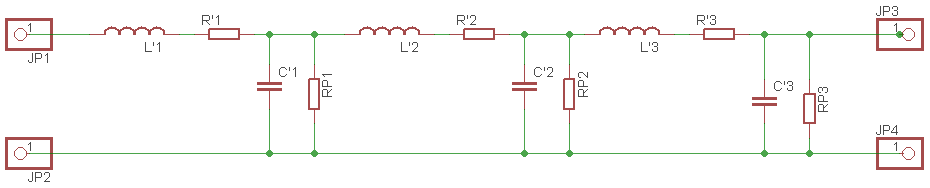
\includegraphics[scale=0.65]{e10/wellenesbex.png}\\
Abb. 7: Genaues Ersatzschaltbild eines Koxialkabels
\end{frame}

\begin{frame}
\frametitle{Wellenwiderstand}
\begin{itemize}
	\item \Huge{ $Z_W = \sqrt{\frac{L'}{C'}}$}
	 \normalsize \item Paralleldrahtleitungen: Zw = 150 $\Omega$ bis 600 $\Omega$
	\item Koaxialleitungen: Zw =  50 $\Omega$ bis 95 $\Omega$
	\item Der Wellenwiderstand entspricht dem Abschlusswiderstand einer Leitung, bei dem keine stehenden Wellen auftreten.
\end{itemize}
\end{frame}

\section*{D\"ampfungsberechnung}
\begin{frame}
\frametitle{D\"ampfungsberechnung}
\begin{Large}
Ich hoffe ihr habt eure Formelsammlung dabei C:
\end{Large}
\end{frame}

\begin{frame}
\frametitle{Let's calculate together}
 \begin{itemize}
 	\item RG58\\
 	\item 40 m\\
 	\item 28 MHz
 \end{itemize}
\end{frame}

\begin{frame}
\frametitle{Let's calculate together}
 \begin{itemize}
 	\item Aircell7\\
 	\item 40 m\\
 	\item 28 MHz
 \end{itemize}
\end{frame}

\begin{frame}
\frametitle{Let's calculate together}
 \begin{itemize}
 	\item RG174\\
 	\item 40 m\\
 	\item 28 MHz
 \end{itemize}
\end{frame}


\section*{Anpassung}
\begin{frame}
\frametitle{Anpassung}
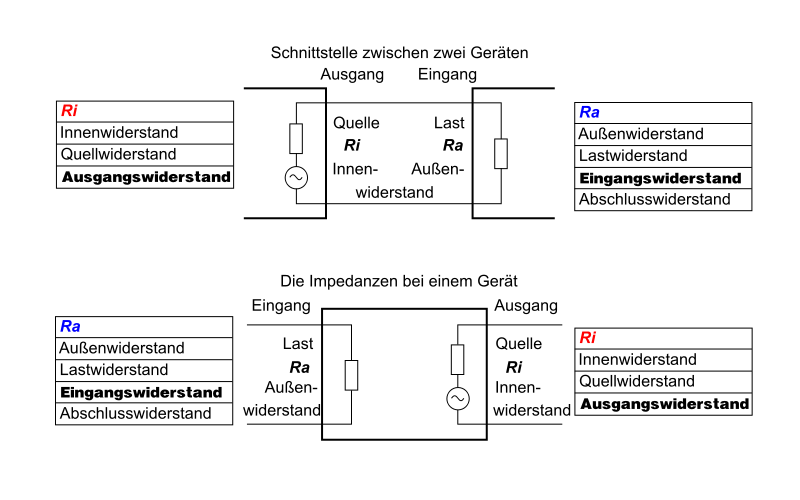
\includegraphics[scale=0.35]{e10/Anpassung.png}\\
Abb. 8: Anpassung
\footnote{\url{http://de.wikipedia.org/wiki/Datei:EingangswiderstandAusgangswiderstandA.svg}}
\end{frame}

\section*{Stehwellenverh\"altnis}
\begin{frame}
\frametitle{Stehwellenverh\"altnis}
\begin{Large}
\begin{itemize}
	\item ist ein Maß für die Anpassung
	\item \Huge $SWR = \frac{u_{v}+u_{r}}{u_{v}-u_{r}}$ \Large
	\item ist das Verhältnis von vorlaufender zu zurücklaufender Welle
	\item \href{http://commons.wikimedia.org/wiki/File:Stehwelle_(Animation).gif}{Animierte Darstellung}
\end{itemize}
\end{Large}
\end{frame}

\section*{Symmetrierung}
\begin{frame}
\frametitle{Symmetrierung}
\begin{minipage}{0.3\textwidth}
	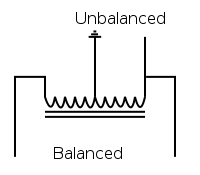
\includegraphics[scale=0.5]{e10/balun.png}\\
	Abb. 9: Balun

\end{minipage}
	\footnote{\url{http://commons.wikimedia.org/wiki/File:Cdbalun2.svg}}
\begin{minipage}{0.6\textwidth}
	\begin{itemize}
		\item Wird bei Verbindungen zwischen symmetrischen und unsymmetrischen Punkten verwendet
		\item Koaxialkabel ist unsymmetrisch
		\item Paralleldraht ist symmetrisch
		\item Alle Dipole sind symmetrisch
		\item Alle Antennen die gegen Erde erregt werden sind unsymmetrisch
	\end{itemize}
\end{minipage}
\end{frame}

\section*{Stecker und Adapter}
\begin{frame}
\frametitle{Stecker und Adapter}
\begin{center}
	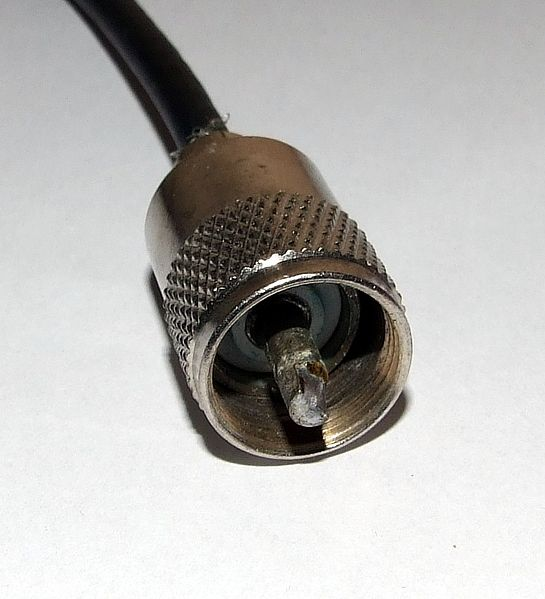
\includegraphics[scale=0.25]{e10/pl.jpg}\\
	Abb. 10: PL-Stecker
	\begin{itemize}
		\item UHF
		\item Kurzwelle,auch 2-Meter-Band
	\end{itemize}
	\footnote{\url{http://de.wikipedia.org/wiki/Datei:UHF_PL_Connector.jpg}}
\end{center}
\end{frame}

\begin{frame}
\frametitle{Stecker und Adapter}
\begin{center}
	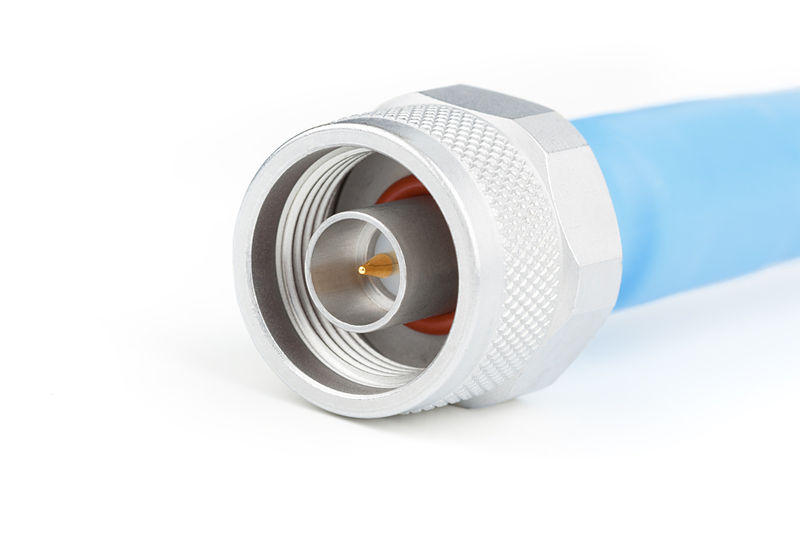
\includegraphics[scale=0.3]{e10/n.jpg}\\
	Abb. 11: N-Stecker
	\begin{itemize}
		\item N
		\item 70-cm-Band, auch 2-Meter-Band
	\end{itemize}	 
	\footnote{\url{http://de.wikipedia.org/wiki/	Datei:Male_type_N_connector.jpg}}
\end{center}
\end{frame}

\begin{frame}
\frametitle{Stecker und Adapter}
\begin{center}
	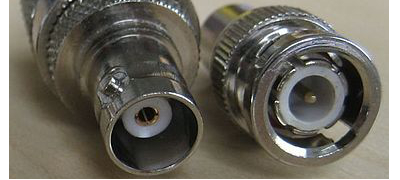
\includegraphics[scale=0.5]{e10/bnc.jpg}\\
	Abb. 12: BNC-Stecker und -Buchse
	\begin{itemize}
		\item BNC
		\item Kurzwelle,auch 2-Meter-Band
	\end{itemize}	
	\footnote{\url{http://commons.wikimedia.org/wiki/File:BNC_50_75_Ohm.jpg}}

\end{center}
\end{frame}

\begin{frame}
\frametitle{Stecker und Adapter}
\begin{center}
	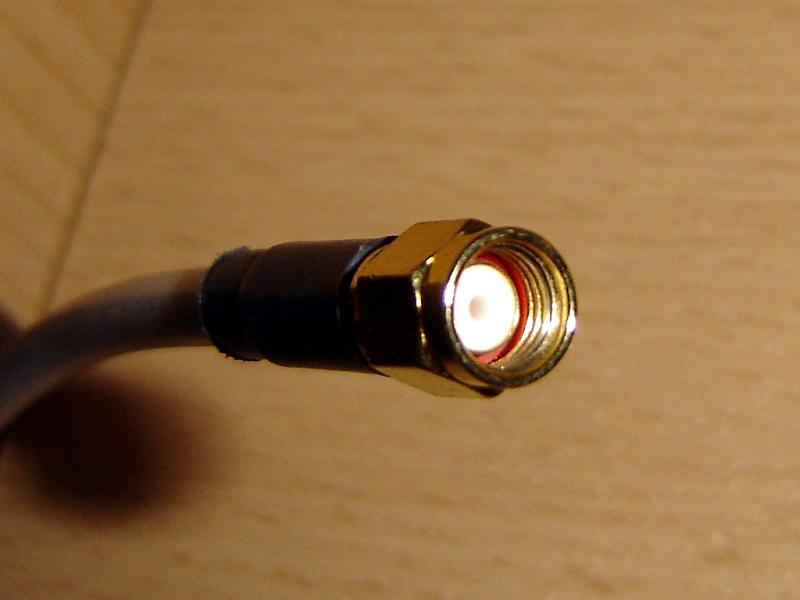
\includegraphics[scale=0.25]{e10/sma.jpg}\\
	Abb. 13: SMA-Stecker
	\begin{itemize}
		\item SMA
		\item VHF-/UHF- Handfunkgeräte
	\end{itemize}	 
	\footnote{\url{http://de.wikipedia.org/wiki/Datei:Reverse_sma_stecker.jpg}}
\end{center}
\end{frame}

\section*{Referenzen}
\begin{frame}
    \frametitle{Referenzen/Links}
    
    \footnotesize
    \begin{itemize}
        \item Moltrecht E 08 : \\
              \url{http://www.darc.de/referate/ajw/ausbildung/darc-online-lehrgang/technik-klasse-e/technik-e08/}      
    \end{itemize}

\end{frame}

% Hier könnte noch eine Kontaktfolie stehen

\end{document}

